\documentclass{article}\usepackage[]{graphicx}\usepackage[]{xcolor}
% maxwidth is the original width if it is less than linewidth
% otherwise use linewidth (to make sure the graphics do not exceed the margin)
\makeatletter
\def\maxwidth{ %
  \ifdim\Gin@nat@width>\linewidth
    \linewidth
  \else
    \Gin@nat@width
  \fi
}
\makeatother

\definecolor{fgcolor}{rgb}{0.345, 0.345, 0.345}
\newcommand{\hlnum}[1]{\textcolor[rgb]{0.686,0.059,0.569}{#1}}%
\newcommand{\hlsng}[1]{\textcolor[rgb]{0.192,0.494,0.8}{#1}}%
\newcommand{\hlcom}[1]{\textcolor[rgb]{0.678,0.584,0.686}{\textit{#1}}}%
\newcommand{\hlopt}[1]{\textcolor[rgb]{0,0,0}{#1}}%
\newcommand{\hldef}[1]{\textcolor[rgb]{0.345,0.345,0.345}{#1}}%
\newcommand{\hlkwa}[1]{\textcolor[rgb]{0.161,0.373,0.58}{\textbf{#1}}}%
\newcommand{\hlkwb}[1]{\textcolor[rgb]{0.69,0.353,0.396}{#1}}%
\newcommand{\hlkwc}[1]{\textcolor[rgb]{0.333,0.667,0.333}{#1}}%
\newcommand{\hlkwd}[1]{\textcolor[rgb]{0.737,0.353,0.396}{\textbf{#1}}}%
\let\hlipl\hlkwb

\usepackage{framed}
\makeatletter
\newenvironment{kframe}{%
 \def\at@end@of@kframe{}%
 \ifinner\ifhmode%
  \def\at@end@of@kframe{\end{minipage}}%
  \begin{minipage}{\columnwidth}%
 \fi\fi%
 \def\FrameCommand##1{\hskip\@totalleftmargin \hskip-\fboxsep
 \colorbox{shadecolor}{##1}\hskip-\fboxsep
     % There is no \\@totalrightmargin, so:
     \hskip-\linewidth \hskip-\@totalleftmargin \hskip\columnwidth}%
 \MakeFramed {\advance\hsize-\width
   \@totalleftmargin\z@ \linewidth\hsize
   \@setminipage}}%
 {\par\unskip\endMakeFramed%
 \at@end@of@kframe}
\makeatother

\definecolor{shadecolor}{rgb}{.97, .97, .97}
\definecolor{messagecolor}{rgb}{0, 0, 0}
\definecolor{warningcolor}{rgb}{1, 0, 1}
\definecolor{errorcolor}{rgb}{1, 0, 0}
\newenvironment{knitrout}{}{} % an empty environment to be redefined in TeX

\usepackage{alltt}
\usepackage[margin=1in]{geometry}
\usepackage{graphicx}
\usepackage{booktabs}
\usepackage{amsfonts} 
\usepackage{amsmath} 
\usepackage{amsthm}
\usepackage{mdframed} 

\newenvironment{boxedproof}[1][Proof]
  {\begin{mdframed}\begin{proof}[#1]}
  {\end{proof}\end{mdframed}}
\usepackage[numbers,sort&compress]{natbib} % For professional numerical citations

\bibliographystyle{plainnat}  

\newcommand{\E}[2][]{\mathbb{E}_{#1}\left[#2\right]}
\newcommand{\Var}[2][]{\mathrm{Var}_{#1}\left(#2\right)}
\newcommand{\Prob}[1]{\mathbb{P}\left(#1\right)}

\title{EUII with Dual Criterion and Bayesian Design}
\author{Saverio Fontana}
\IfFileExists{upquote.sty}{\usepackage{upquote}}{}
\begin{document}    
\maketitle   
  


\section*{Dual Criterion with a frequentist approach}
\subsection{Fixed Design}
\textit{Here you should put the EUII calculation for Dual criterion fixed design}
TO DO 
Implement this in the example from "Beyond p-values: a phase II dual-criterion design with statistical significance and clinical relevance" on
Hazard Ratios.

\subsection{Sequential Design}
What about using sequential design in a frequentist framwork with dual criterion? I didn't find any examples of that anywhere


\section*{Dual Criterion with a bayesian approach}


Now we reproduce \textbf{Example 3.1} from the paper from Gsponer \cite{gsponer2014bayesian}

\begin{knitrout}
\definecolor{shadecolor}{rgb}{0.969, 0.969, 0.969}\color{fgcolor}\begin{kframe}
\begin{alltt}
\hldef{design} \hlkwb{<-} \hlkwd{gsbDesign}\hldef{(}\hlkwc{nr.stages} \hldef{=} \hlnum{2}\hldef{,}
                    \hlkwc{patients} \hldef{=} \hlkwd{c}\hldef{(}\hlnum{10}\hldef{,}\hlnum{20}\hldef{),}
                    \hlkwc{sigma}\hldef{=}\hlnum{88}\hldef{,}
                    \hlkwc{criteria.success} \hldef{=} \hlkwd{c}\hldef{(}\hlnum{0}\hldef{,}\hlnum{0.95}\hldef{,}\hlnum{50}\hldef{,}\hlnum{0.5}\hldef{),}
                    \hlkwc{criteria.futility} \hldef{=} \hlkwd{c}\hldef{(}\hlnum{40}\hldef{,}\hlnum{0.9}\hldef{),}
                    \hlkwc{prior.control} \hldef{=} \hlkwd{c}\hldef{(}\hlnum{49}\hldef{,}\hlnum{20}\hldef{),}
                    \hlkwc{prior.treatment} \hldef{=} \hlkwd{c}\hldef{(}\hlnum{49}\hldef{,}\hlnum{0}\hldef{))}
\end{alltt}
\end{kframe}
\end{knitrout}

\begin{knitrout}
\definecolor{shadecolor}{rgb}{0.969, 0.969, 0.969}\color{fgcolor}\begin{kframe}
\begin{alltt}
\hldef{simulation} \hlkwb{<-} \hlkwd{gsbSimulation}\hldef{(}
  \hlkwc{truth}\hldef{=}\hlkwd{list}\hldef{(}\hlnum{49}\hldef{,}\hlkwd{c}\hldef{(}\hlnum{0}\hldef{,}\hlnum{40}\hldef{,}\hlnum{50}\hldef{,}\hlnum{60}\hldef{,}\hlnum{70}\hldef{)),}
  \hlkwc{grid.type}\hldef{=}\hlsng{"sliced"}\hldef{,}
  \hlkwc{method} \hldef{=} \hlsng{"both"}\hldef{,}
  \hlkwc{type.update}\hldef{=}\hlsng{"per arm"}\hldef{,}
  \hlkwc{nr.sim}\hldef{=}\hlnum{100000}\hldef{,}
  \hlkwc{warnings.sensitivity} \hldef{=} \hlnum{500}\hldef{,}
  \hlkwc{seed}\hldef{=}\hlnum{1}\hldef{)}
\end{alltt}
\end{kframe}
\end{knitrout}

\begin{knitrout}
\definecolor{shadecolor}{rgb}{0.969, 0.969, 0.969}\color{fgcolor}\begin{kframe}
\begin{alltt}
\hldef{result_new} \hlkwb{<-} \hlkwd{gsb}\hldef{(}\hlkwc{design}\hldef{=design,}\hlkwc{simulation}\hldef{=simulation)}
\end{alltt}
\end{kframe}
\end{knitrout}

To extract the results, we use \texttt{what = "cumulative all"} to obtain the cumulative probabilities of success and futility across stages.

\begin{knitrout}
\definecolor{shadecolor}{rgb}{0.969, 0.969, 0.969}\color{fgcolor}\begin{kframe}
\begin{alltt}
\hldef{table_total} \hlkwb{<-} \hlkwd{tab}\hldef{(result_new,} \hlkwc{what} \hldef{=} \hlsng{"cumulative all"}\hldef{)}
\hldef{table_n} \hlkwb{<-} \hlkwd{tab}\hldef{(result_new,} \hlkwc{what} \hldef{=} \hlsng{"sample size"}\hldef{)}
\hldef{T1E} \hlkwb{<-} \hldef{table_total[}\hlnum{1}\hldef{,} \hlsng{"stage2.suc"}\hldef{]}
\hldef{powers} \hlkwb{<-} \hldef{table_total[}\hlnum{2}\hlopt{:}\hlnum{5}\hldef{,} \hlkwd{c}\hldef{(}\hlsng{"delta"}\hldef{,} \hlsng{"stage2.suc"}\hldef{)]}
\end{alltt}
\end{kframe}
\end{knitrout}

The Type I error rate is $\mathit{T1E} = \Prob{+|H_0} = 1.2\%$.

% latex table generated in R 4.5.2 by xtable 1.8-8 package
% Fri Mar 13 14:03:28 2026
\begin{table}[h]
\centering
\begin{tabular}{rr}
  \hline
delta & stage2.suc \\ 
  \hline
40.00 & 0.41 \\ 
  50.00 & 0.63 \\ 
  60.00 & 0.81 \\ 
  70.00 & 0.93 \\ 
   \hline
\end{tabular}
\caption{Power at various effect sizes} 
\end{table}


\vspace{0.5cm}
\noindent \textbf{Note on notation:}
\begin{itemize}
    \item \textbf{+} means we reject the null hypothesis (\textit{success}).
    \item \textbf{-} means we fail to reject the null (currently including both No-Go and Inconclusive outcomes). 
\end{itemize}

\textbf{SEE the end for discussion about this}




\section*{Likelihood Ratios and Information Indices}

We define the Positive Likelihood Ratio ($LR_+$) and Negative Likelihood Ratio ($LR_-$) as:

\begin{equation}
    LR_+ = \frac{\mathit{Power}}{\mathit{T1E}} = \frac{\Prob{+|H_1}}{\Prob{+|H_0}}
\end{equation}

\begin{equation} 
    LR_- = \frac{1 - \mathit{Power}}{1 - \mathit{T1E}} = \frac{\Prob{-|H_1}}{\Prob{-|H_0}}
\end{equation}

The Diagnostic Odds Ratio ($DOR$), is:
\begin{equation}
    DOR = \frac{LR_+}{LR_-}
\end{equation}

\begin{knitrout}
\definecolor{shadecolor}{rgb}{0.969, 0.969, 0.969}\color{fgcolor}\begin{kframe}
\begin{alltt}
\hldef{LR_pos} \hlkwb{<-} \hlkwd{cbind}\hldef{(powers[,}\hlsng{"delta"}\hldef{], powers[,} \hlsng{"stage2.suc"}\hldef{]} \hlopt{/} \hldef{T1E)}
\hldef{LR_neg} \hlkwb{<-} \hlkwd{cbind}\hldef{(powers[,}\hlsng{"delta"}\hldef{], (}\hlnum{1} \hlopt{-} \hldef{powers[,} \hlsng{"stage2.suc"}\hldef{])} \hlopt{/} \hldef{(}\hlnum{1} \hlopt{-} \hldef{T1E))}
\hldef{DOR} \hlkwb{<-} \hlkwd{cbind}\hldef{(}\hlkwc{delta} \hldef{= LR_pos[,} \hlnum{1}\hldef{],} \hlkwc{DOR} \hldef{= LR_pos[,} \hlnum{2}\hldef{]} \hlopt{/} \hldef{LR_neg[,} \hlnum{2}\hldef{])}
\end{alltt}
\end{kframe}
\end{knitrout}

\begin{figure}[h]
\centering
\begin{knitrout}
\definecolor{shadecolor}{rgb}{0.969, 0.969, 0.969}\color{fgcolor}
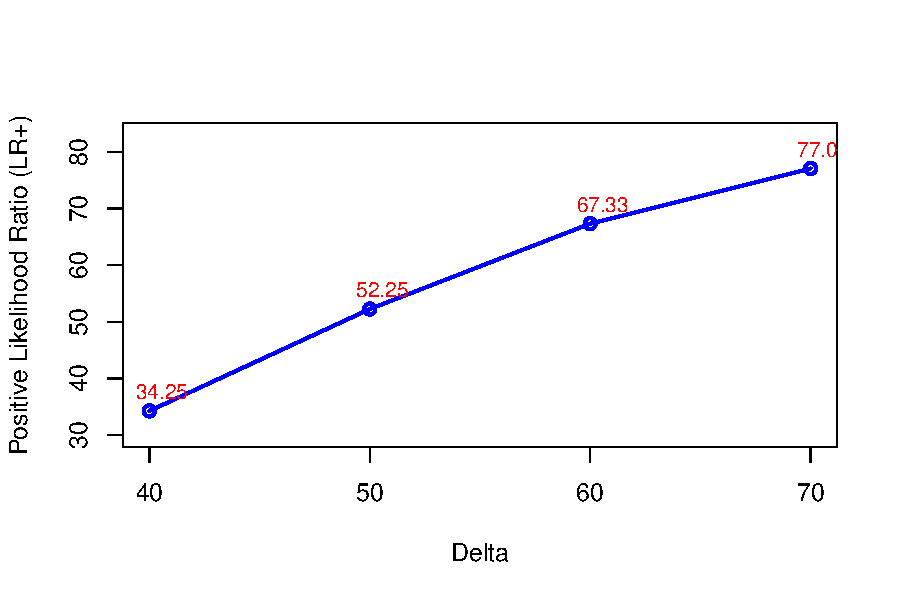
\includegraphics[width=\maxwidth]{figure/lr-pos-plot-1} 
\end{knitrout}
\caption{Positive Likelihood Ratio vs Delta}
\end{figure}


\begin{knitrout}
\definecolor{shadecolor}{rgb}{0.969, 0.969, 0.969}\color{fgcolor}\begin{figure}[h]
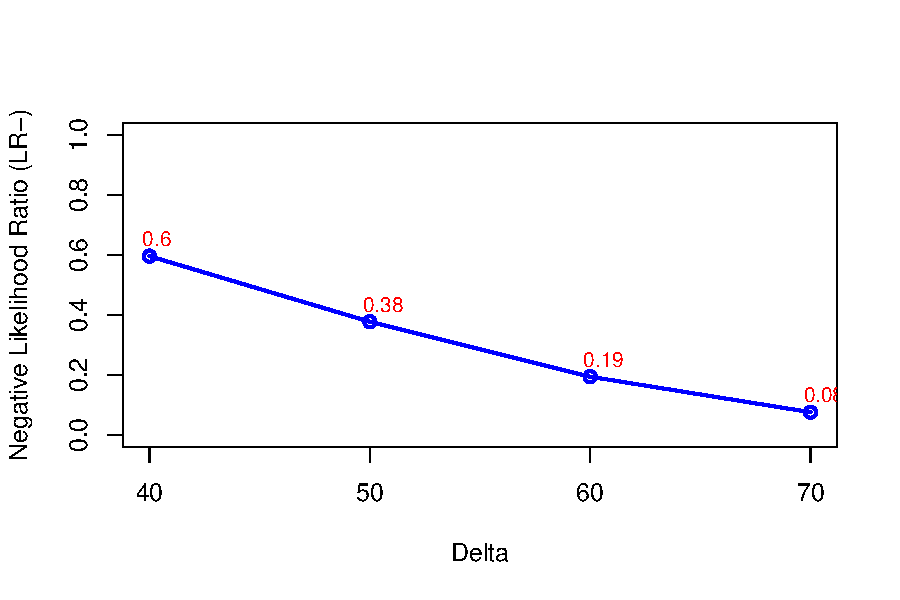
\includegraphics[width=\maxwidth]{figure/lr-neg-plot-1} \caption[Negative Likelihood Ratio vs Delta]{Negative Likelihood Ratio vs Delta}\label{fig:lr-neg-plot}
\end{figure}

\end{knitrout}


% latex table generated in R 4.5.2 by xtable 1.8-8 package
% Fri Mar 13 14:03:28 2026
\begin{table}[h]
\centering
\begin{tabular}{rr}
  \hline
delta & DOR \\ 
  \hline
40.00 & 57.45 \\ 
  50.00 & 138.40 \\ 
  60.00 & 346.49 \\ 
  70.00 & 1015.44 \\ 
   \hline
\end{tabular}
\caption{DOR at various effect sizes} 
\end{table}


\clearpage

\section*{Experimental Unit Information Index (EUII)}

The (first-order) Experimental Unit Information Index (EUII) is:

\begin{equation}
    EUII \approx \frac{LR_+^{1/\E{N_+}}}{LR_-^{1/\E{N_-}}}
\end{equation}

It is important to notice that \texttt{gsbDesign} only provides $\E{N|H_1}$ and $\E{N|H_0}$, 
but with a bit of calculation we can get $\E{N_+}$ and $\E{N_-}$.\\ 

Define $n_j$ the sample size we'd have if we stop at stage $j$. 
\textit{We only have $n_1$ and $n_2$ in this example, respectively 30 and 60, since we have 10 placebo and 20 tratments each step.} \\ 


Denote $\E{N  \mid +} := \E{N_+} = \E{\text{sample size} \mid \text{success}}$, which is the expected sample size given that the trial ends in a rejection (\textit{success}). 

Similarly, $\E{N  \mid +, H_0 } := \E{N_{0+}} = \E{\text{sample size} \mid \text{success under } H_0}$ is the expected sample size given a successful result, assuming the Null is true. \\

We can then use the formula of the Expected Value:
$$ \E{N  \mid +, H_0} = n_1 \times \Prob{\text{stop at 1} \mid +, H_0} + n_2 \times \Prob{\text{stop at 2} \mid +, H_0} $$
where:
$$ \Prob{\text{stop at } i \mid +, H_0} = \frac{\Prob{\text{success at } i \mid H_0}}{\Prob{\text{success at 1 or 2} \mid H_0}} $$

Next, we need the posterior probabilities $\Prob{H_0  \mid +}$ and $\Prob{H_1  \mid +}$. Those can be obtained using the property of $LR_+$:
$$ Odds(H_1  \mid +) = LR_+ \times Odds(H_1) $$ 
where the prior odds are $Odds(H_1) = \frac{\Prob{H_1}}{1 - \Prob{H_1}}$ and we need to specify $\Prob{H_1}$ (\textit{usually $\{0.01, 0.1, 0.5\}$})
 
We then back-transform the Odds into a Probability:
$$ \Prob{H_1  \mid +} = \frac{Odds(H_1  \mid +)}{1 + Odds(H_1  \mid +)} $$
and simply obtain $\Prob{H_0  \mid +} = 1 - \Prob{H_1  \mid +}$.

Finally, we apply the law of total expectation to find the overall expected sample size for a significant result:
$$ \E{N  \mid +} = \E{N  \mid +, H_0} \times \Prob{H_0  \mid +} + \E{N  \mid +, H_1} \times \Prob{H_1  \mid +} $$

An analogous method is used to obtain $\E{N  \mid -}$ for nonsignificant results.\\
 





\begin{knitrout}
\definecolor{shadecolor}{rgb}{0.969, 0.969, 0.969}\color{fgcolor}
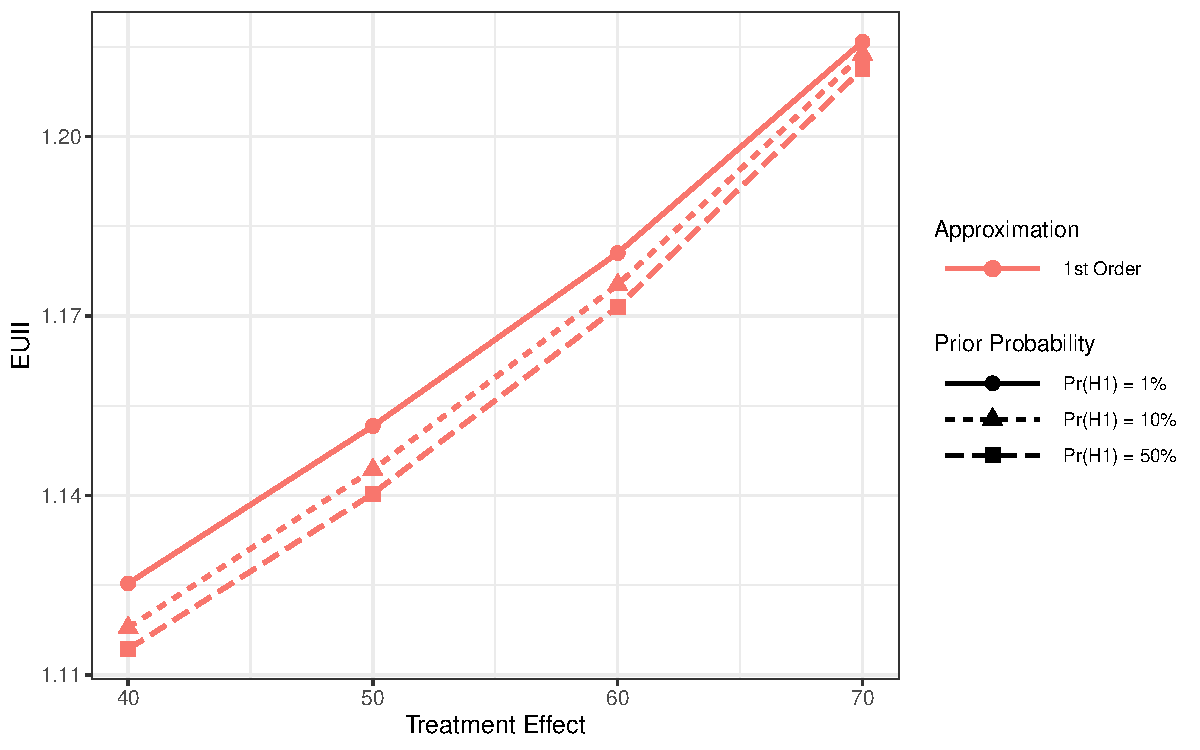
\includegraphics[width=\maxwidth]{figure/first_order_euii-1} 
\end{knitrout}


\subsection{Second order EUII}
\label{sec: second order}
Now we compute the second-order approximation of the EUII

First, we calculate the second moments and conditional variances of the sample size under each hypothesis. For a significant result ($+$) under $H_0$:
$$ \E{N_{0+}^2} = n_1^2 \times \Prob{\text{stop at 1} \mid +, H_0} + n_2^2 \times \Prob{\text{stop at 2} \mid +, H_0} $$
Using then the formula for the Variance: $$ Var(N_{0+}) = \E{N_{0+}^2} - [\E{N_{0+}}]^2 $$
The conditional variance $Var(N_{1+})$ under $H_1$ is computed analogously.

Next, we calculate the overall variance $Var(N_+)$ using the Law of Total Variance, (Equation 18 paper):
\begin{align*}
Var(N_+) &= \left( Var(N_{0+}) \Prob{H_0 \mid +} + Var(N_{1+}) \Prob{H_1 \mid +} \right) \\
&\quad + \left( [\E{N_{0+}} - \E{N_+}]^2 \Prob{H_0 \mid +} + [\E{N_{1+}} - \E{N_+}]^2 \Prob{H_1 \mid +} \right)
\end{align*}

We then compute the Coefficient of Variation for significant findings:
$$ CV(N_+) = \frac{\sqrt{Var(N_+)}}{\E{N_+}} $$

Repeating this entire process for nonsignificant findings ($-$) gives $CV(N_-)$. \\

Now we can compute the 2-nd order EUII: 
$$ EUII_{2nd} = \frac{(LR^+)^{(1 + CV(N_+)^2) / \E{N_+}}}{(LR^-)^{(1 + CV(N_-)^2) / \E{N_-}}} $$
 
\begin{knitrout}
\definecolor{shadecolor}{rgb}{0.969, 0.969, 0.969}\color{fgcolor}
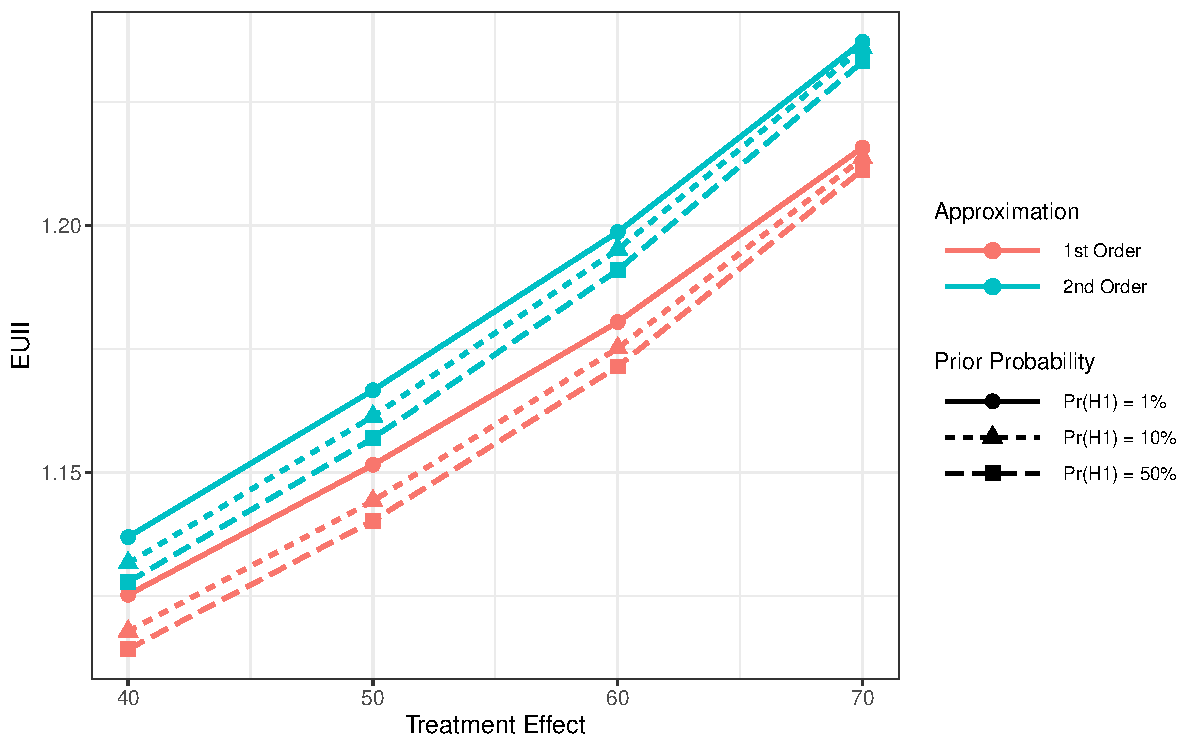
\includegraphics[width=\maxwidth]{figure/second_order_euii-1} 
\end{knitrout}

\subsection{Exact calculation of EUII}
In group sequential design, we cannot compute $\log(EUII)$ directly, since N is a random variable. 
In the EUII paper \cite{held2025euii} they propose to compute $\E[]{\log(EUII)} = \E{\frac{1}{N_+}} \log{LR_+} - \E{\frac{1}{N_-}} \log{LR_-}$.

A first order approximation is proposed: $\E{\frac{1}{N_+}} \approx \frac{1}{\E{N_+}}$. And as 
we have seen, they also suggest a second order approximation.     \\
I suggest instead to compute $$\exp(\E{\log(EUII)}) = (LR_+)^{\E{\frac{1}{N_+}}} \times \left(\frac{1}{LR_-}\right)^{\E{\frac{1}{N_-}}} $$ 
Where $\E{\frac{1}{N_+}}$ is computed using the definition of Expected Value:
\[  \E{\frac{1}{N_+}} = \frac{1}{n_1} \times \Prob{\text{stop at 1} \mid +} + \frac{1}{n_2} \times \Prob{\text{stop at 2}  \mid +} \]





Now I will prove that my version is always greater than the first order approximation.


\begin{boxedproof}
$f(x) = \frac{1}{x}$ is a strictly convex function for $x>0$. So we can apply Jensen's Inequality:
\[ \frac{1}{\E{N_+}} \le \E{\frac{1}{N_+}}  \]
We can then assume wlog Power $\geq$ Type I Error, meaning $LR_+ > 1$ and $LR_- < 1$ (otherwise we'd have a nonsensical design) \\
Consequently, both $\log(LR_+) > 0$ and $\log\left(\frac{1}{LR_-}\right) > 0$ and we can write:
\[\E[]{\log(EUII)} =  \E{\frac{1}{N_+}} \log{LR_+} + \E{\frac{1}{N_-}} \log{\frac{1}{LR_-}} \geq 
\frac{1}{\E{N_+}} \log{LR_+} + \frac{1}{\E{N_-}} \log{\frac{1}{LR_-}}\]

then if we take the $exp()$ both sides, inequality is preserved since it is a monotonic increasing function:
\[ \exp(\E{\frac{1}{N_+}} \log{LR_+}) \times \exp(\E{\frac{1}{N_-}} \log{\frac{1}{LR_-}}) \geq 
\exp(\frac{1}{\E{N_+}} \log{LR_+}) \times  \exp(\frac{1}{\E{N_-}} \log{\frac{1}{LR_-}}) \]
Finally simplifying:
\[ \underbrace{(LR_+)^{\E{\frac{1}{N_+}}} \times \left(\frac{1}{LR_-}\right)^{\E{\frac{1}{N_-}}}}_{\exp(\E{\log(EUII)})} \geq 
\underbrace{(LR_+)^{\frac{1}{\E{N_+}}} \times \left(\frac{1}{LR_-}\right)^{\frac{1}{\E{N_-}}}}_{EUII_{1st}}\]


\end{boxedproof}



\textbf{NOTE:} in Figure~\ref{fig:exact_EUII}, I plotted $\exp(\E{\log(EUII)})$  and I call it \textit{"exact"}. I think we should use this metric instead of $\E{EUII}$,
cause $\E[]{\log(EUII)}$ has an interpretation in information theory, while $\E{EUII}$ doesn't. \\
Actually, this is something I'd like to go deeper on, since I think it is possible to justify better the EUII using Entropy or something related\\

Anyway, applying Jensen since $h(x) = \exp(x)$ is strictly convex, we get:
\[
\E{EUII} = \E{\exp(\log EUII)} \geq \exp\left(\E{\log(EUII)}\right)
\]
 

I also think it would be possible to compute $\E{EUII}$, even though I haven't implemented it.
First, the expected value of a product of independent variables is the product of their expected values: 
\[ \E{EUII} = \E{(LR_+)^{1/N_+}} \times \E{\left(\frac{1}{LR_-}\right)^{1/N_-}}\]


where the first term is:
\[ \E{(LR_+)^{1/N_+}} = \left( (LR_+)^{1/n_1} \times \Prob{\text{stop at 1} \mid +} \right) + \left( (LR_+)^{1/n_2} \times \Prob{\text{stop at 2} \mid +} \right) \]
and the second term is:
\[\E{\left(\frac{1}{LR_-}\right)^{1/N_-}} = \left( \left(\frac{1}{LR_-}\right)^{1/n_1} \times \Prob{\text{stop at 1} \mid -} \right) + \left( \left(\frac{1}{LR_-}\right)^{1/n_2} \times \Prob{\text{stop at 2} \mid -} \right)\]

\bigskip
Finally, looking at Figure~\ref{fig:exact_EUII}, the exact version is smaller than the 2nd Order, probably due to the fact we are missing the correction of the third order term, which is subtracted. 
$$E[\frac{1}{N}] \approx \frac{1}{\mu} + \frac{Var(N)}{\mu^3} - \underbrace{\frac{E[(N-\mu)^3]}{\mu^4}}_{\text{missing term}}
 + \dots$$


\begin{knitrout}
\definecolor{shadecolor}{rgb}{0.969, 0.969, 0.969}\color{fgcolor}\begin{figure}
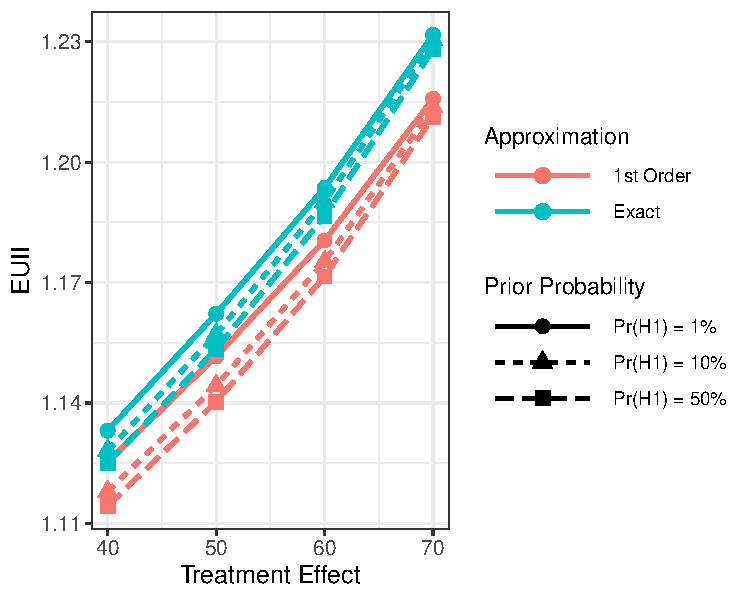
\includegraphics[width=0.49\textwidth]{figure/exact_EUII-1} 
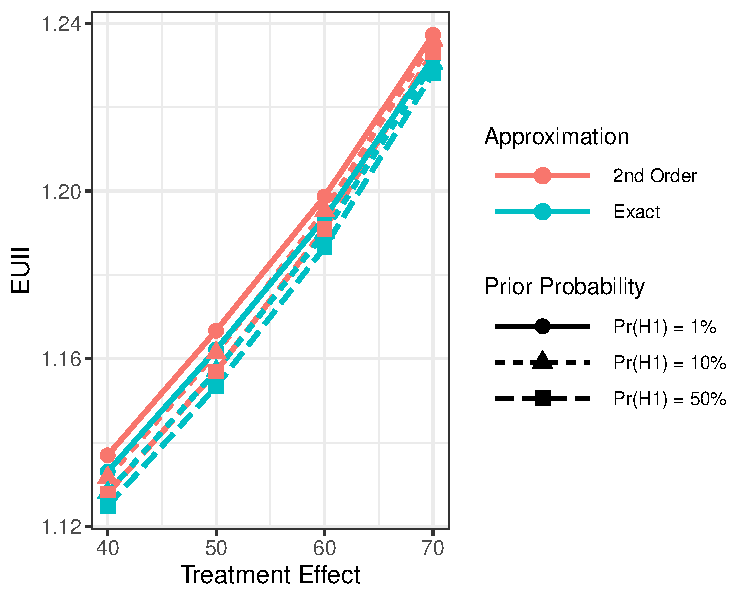
\includegraphics[width=0.49\textwidth]{figure/exact_EUII-2} \caption[comparison of approx with exact EUII]{comparison of approx with exact EUII.}\label{fig:exact_EUII}
\end{figure}

\end{knitrout}

\newpage

\section{Comparison with fixed design and non informative prior (all 4 combinations)}
Now we do the plot that was in the Preliminary paper but was wrong. 
Denote as $n_{virtual}$ the virtual sample size due to the prior

Basically we inspect 4 variants of the same experiment from GSPONER:
\begin{itemize}
  \item sequential design with 2 groups with 10 placebo and 20 treatments per group with a $n_{virtual} = 20$
  \item sequential design with 2 groups with 20 placebo and 20 treatments per group and uninformative prior
  \item fixed design with 60 patients and $n_{virtual} = 20$
  \item fixed design with 80 patients and uninformative prior
\end{itemize}

\begin{knitrout}
\definecolor{shadecolor}{rgb}{0.969, 0.969, 0.969}\color{fgcolor}
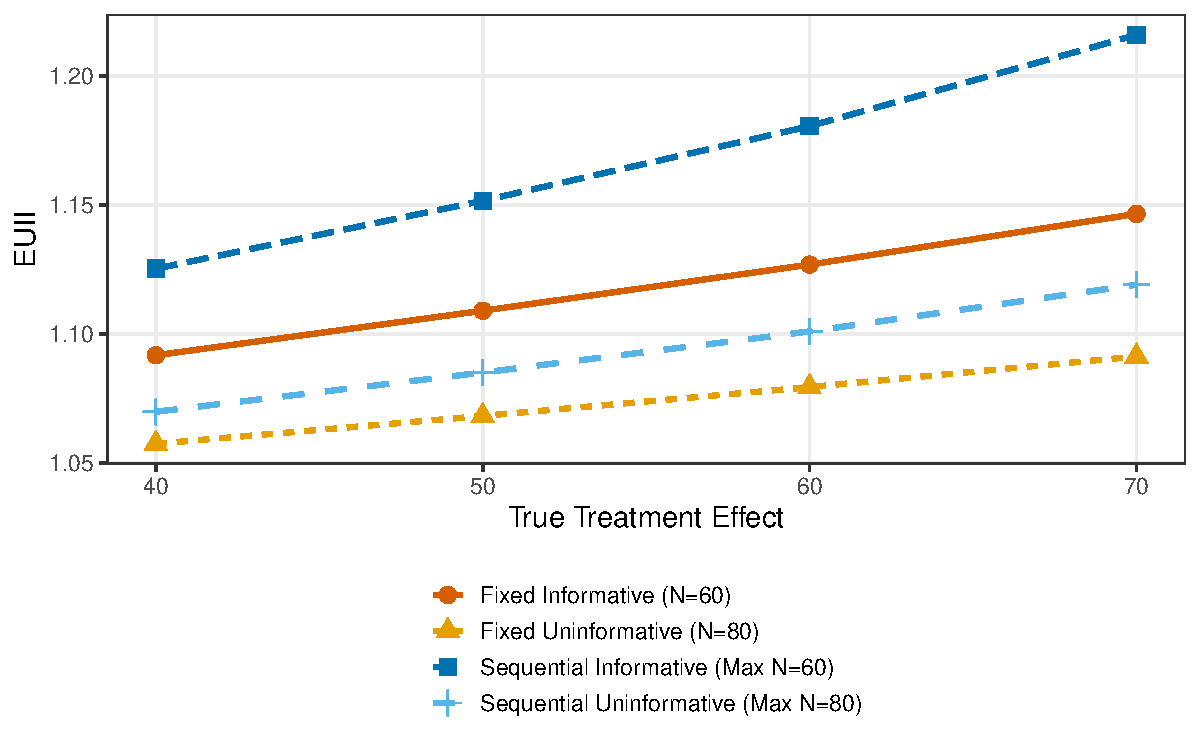
\includegraphics[width=\maxwidth]{figure/4cases-1} 
\end{knitrout}


 \subsection{Adapting sample size for bayesian}

 I kind of argue that it doesn't make sense to add to N the virtual sample size of the prior. \\
My idea is that each new animal is more "valuable" because its data is strenghtened by the historical prior. \\
We need to save on animals, and virtual patients cost nothing, they are like free informations



 \subsection{Including or not the indifferent in the -?}

\vspace{0.5cm}
\noindent \textbf{Note on notation:}
\begin{itemize}
    \item \textbf{+} means we reject the null hypothesis (\textit{success}).
    \item \textbf{-} means we fail to reject the null (currently including both No-Go and Inconclusive outcomes). 
\end{itemize}

An idea would also be to consider as a "-" only the No-Go, completing ignoring the indefinite. \\
To me it doesn't make sense much. Here are my points:\\
First, when we use futility stopping in Sequential Testing, reaching the final analysis without rejecting the null hypothesis $H_0$ is treated identically to
 an early futility stop in terms of expected sample size and error rate calculations.\\
Then, just take the COVID example, the vaccines that weren't satisfying the dual 
criterion, were not approved. So any outcome that does not result in a "Go" decision carries 
the same value as a definitive "No-Go". \\
        
     
   
\bibliography{references}   
\end{document} 
  

    
